\section{Lidar Hardware}
The sensor used to detect environmental obstacles was a Hokuyo
URG-04LX-UG01, which can be seen in Figure~\ref{fig:lidar_top1}. 
The URG is a 2D scanning laser rangefinder, more commonly known as
a Lidar. Lidar is a portmanteau for \textit{Li}ght \textit{D}etection 
\textit{a}nd \textit{R}anging and operates using principles similar 
to Radar and Sonar. 2D Lidars provide a number of discrete range measurements
along a plane. This effectively gives a ``top-down'' or ``blue-print''
style view of an environment.
This, when mounted to a robot, allows the detection of objects in one plane of
the environment so that the robot can avoid or plan a path around them.

\begin{figure}
\centering
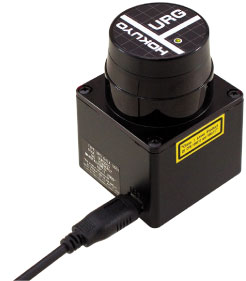
\includegraphics[height=0.3\textheight]{hokuyo/urg_04lx_ug01_top.jpg}
\caption{Photograph of the URG-04LX-UG01 Lidar. It is shown
         with a USB cable plugged in, which is the method of powering
         and retrieving data from the Lidar.}
\label{fig:lidar_top1}
\end{figure}

2D scanning Lidars such as the URG, sense the environment by emitting a laser
beam and measuring the time it takes for the emitted photons to return to the sensor.
This time is used to compute the range to the obstacle that the beam encountered.
Commonly, photons are not actually timed, but rather the phase difference of the
emitted light is used to estimate the time.
Following this measurement, the laser is then mechanically rotated to another 
angular position to take another reading. The process is repeated through the 
entire scanning angle of the sensor, and the set of range-angle pairs is 
considered ``one scan''. The URG uses a spinning mirror to rotate the beam, while
other sensors rotate the entire laser assembly.
An example of the data returned from the URG can be seen in Figure~\ref{fig:lidar_scan1}.
The URG was placed in a hall with a doorway to its left.

\begin{figure}
\centering
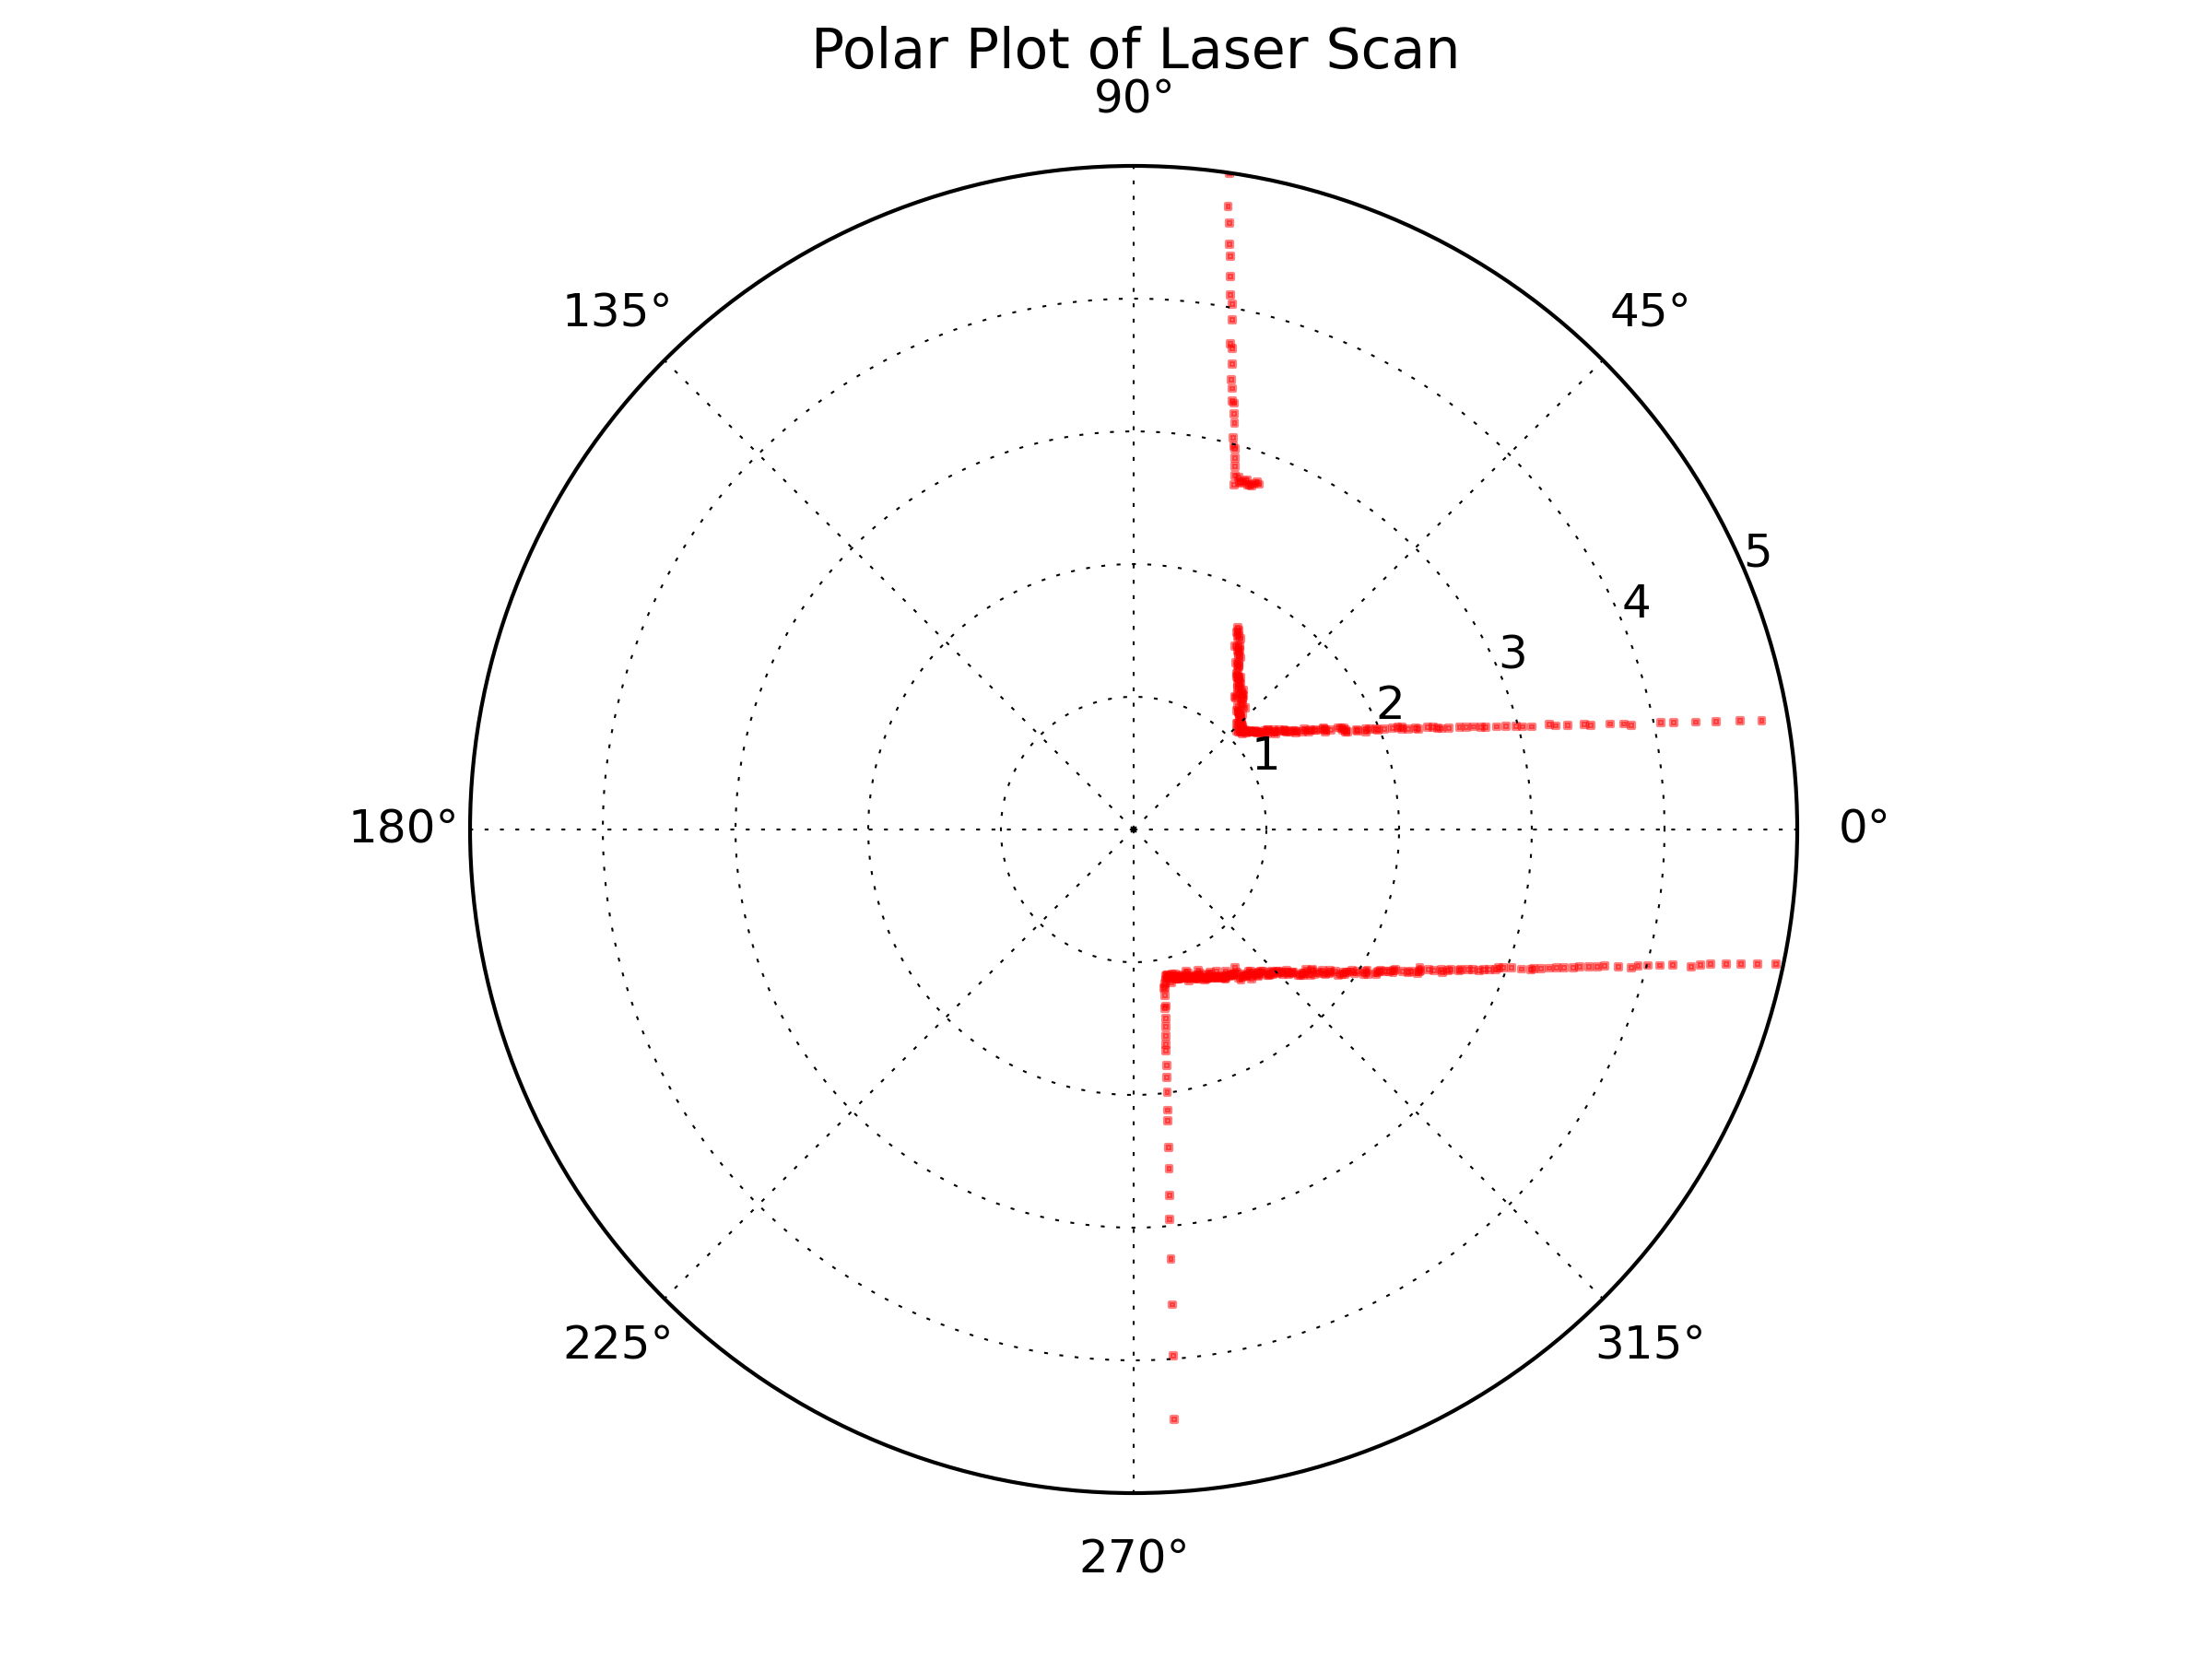
\includegraphics[height=0.4\textheight]{laser_scan_msg2.yaml_1.png}
\caption{Scan from the URG\@.
         The sensor is in the center of the figure.
         The radius of the figure is limited to 5 meters, which is 1 meter 
         greater than the maximum rated range of the sensor. While the unit will
         still provide data at this range, its accuracy is unrated.
         In this scan, the sensor is facing a hall, with a doorway to its left.}
\label{fig:lidar_scan1}
\end{figure}

The URG is a good choice for these experiments due to its lightweight and small
dimensions. This allows it to be easily mounted to the Nao Humanoid while
respecting the payload capacity of the robot. It has a wide scan angle, high
angular resolution, and a good range for this application. A high angular
resolution allows the robot to detect narrow obstacles that might obstruct the
robot's path, yet unlike sonar, provide detailed information about unobstructed
areas the robot can traverse. While the URG is rated for indoor use only, this
is sufficient for our application as the Nao is not often used in outdoor 
situations. Lastly, the sensor can be operated through a single USB port,
sourcing power from and providing data to the robot. This means no additional hardware is 
necessary for the Nao to make use of the sensor, as a USB port is available
in the back of the robot's head.
Figure~\ref{fig:lidar_diagram1} shows a mechanical drawing of the sensor, while
Table~\ref{tab:lidar_params1} lists some of the relevant specifications of the
URG.

\begin{table}
\centering
\begin{tabulary}{\textwidth}{|l||l|r|r|r|l|}
\hline
\textbf{Properties}& \textbf{Condition}         & \textbf{Min} & \textbf{Typ} & \textbf{Max} & \textbf{Units} \\	\hline\hline
\textbf{Scanner}   &                            &              &              &              &                \\	\hline
View Angle 	       &                            &              & 240          &              & degrees        \\	\hline
Angular Resolution &                            &              & 0.36         &              & degrees        \\	\hline
Range 	           &                            & 20           &              & 4000         & mm             \\	\hline 
Linear Resolution  &                            &              & 1            &              & mm             \\	\hline 
Accuracy           & Distance: 20 mm to 1000 mm &              & $\pm$ 30     &              & mm             \\	\hline 
        	       & Distance: 20 mm to 4000 mm &              & $\pm$ 3      &              & \%             \\	\hline \hline 
\textbf{Mechanical}&                            &              &              &              &                \\	\hline
Update Rate	       &                            &              & 100          &              & ms/scan        \\	\hline 
Weight             &                            &              & 160          &              & g              \\	\hline 
Width              &                            &              & 50           &              & mm             \\	\hline 
Length             &                            &              & 50           &              & mm             \\	\hline 
Height             &                            &              & 70           &              & mm             \\	\hline \hline
\textbf{Electrical}&                            &              &              &              &                \\	\hline 
Voltage Rating     &                            & 4.75         & 5.0          & 5.25         & V              \\	\hline 
Current Draw       &                            &              & 500          & 800          & mA             \\	\hline 
\end{tabulary} 
\caption{This table contains various specifications of the Hokuyo URG-04LX-UG01.
         These values were taken from the datasheet of the Lidar, which can be found here~\cite{urg_specs}.}
\label{tab:lidar_params1}
\end{table}

\begin{figure}
\centering
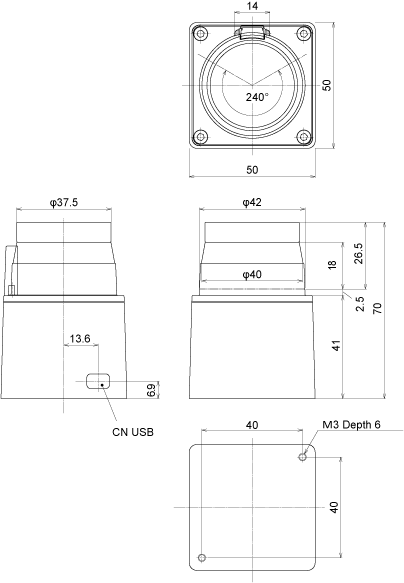
\includegraphics[height=0.3\textheight]{hokuyo/urg_04lx_ug01_ed.png}
\caption{Mechanical drawing of the URG-04LX-UG01.
         The compact size of the URG makes it easy to mount to the Nao.}
\label{fig:lidar_diagram1}
\end{figure}
